\documentclass[fiche]{classe-tex3R}
\usepackage{style-tex3R}

\usepackage{accsupp}

\colorlet{colorBasic}{SlateGrey}
\colorlet{colorBracket}{DarkViolet}
\colorlet{colorKeyword}{DarkBlue}
\colorlet{colorEnvironment}{LightSeaGreen}
\colorlet{colorComment}{Green}
\colorlet{colorString}{DarkOrange}
\colorlet{colorChange}{Red}
\colorlet{colorMath}{Teal}
\colorlet{colorVariable}{LightSkyBlue}
\colorlet{colorBoolean}{Indigo}
\colorlet{colorFunction}{DarkBlue}

\lstset{
  %Réglages généraux
  backgroundcolor=\color{gray!20!white},
  basicstyle=\ttfamily\small\color{colorBasic},
  columns=fullflexible,
  aboveskip=0pt,
  belowskip=0pt,
  breaklines=true,
  %Keywords
  emph={[1]
    begin,
    end,
    documentclass,
    usepackage,
    definirchapitre,
    definirniveau,
    parametrage,
    bareme,
    competence,
    difficulte,
    source,
    theme,
    montitre,
    important,
    tailletexte,
    partie,
    souspartie,
    chapitre,
    visiblecmd,
    saut,
    lignes,
    ifdiapo,
    iffiche,
    ifheader,
    ifprint,
    ifactivite,
    ifbasique,
    ifbilan,
    ifcorrige,
    ifcours,
    ifTD,
    ifflash,
    ifDM,
    ifDS,
    ifinterro,
    ifcorrection,
    ifenonce,
    ifvisible,
    ifbareme,
    ifdifficulte,
    ifcompetence,
    ifsource,
    iftheme,
    ifstretch,
    ifsubfile,
    else,
    fi,
    newcounter,
    setcounter,
    stepcounter,
    thecompteurexercice,
    tkzDefPoints,
    tkzDefMidPoint,
    tkzDrawPoints,
    tkzLabelPoints,
    tkzGetPoint,
    tkzMarkSegments,
    tkzDrawSegments,
    tkzLabelSegments,
    tkzDefLine,
    tkzGetPoints,
    tkzMarkRightAngles,
    tkzDrawLines,
    tkzLabelLine,
    tkzDrawPolygon,
    tkzDefSpcTriangle,
    tkzDefTriangleCenter,
    tkzDrawCircles,
    tkzDefPointWith,
    tkzDrawSemiCircles,
    tkzDefPointOnLine,
    tkzDefPointOnCircle,
    tkzDrawArc,
  }, 
  emphstyle={[1]\color{colorKeyword}},
  %Environnements
  emph={[2]
    environnement,
    luacode,
    fiche,
    document,
    application,
    convention,
    definition,
    exemple,
    methode,
    propriete,
    preuve,
    remarque,
    enonce,
    correction,
    visible,
    tikzpicture
  }, 
  emphstyle={[2]\color{colorEnvironment}},
  %Variable lua
  emph={[3]
  Type,
  Impression,
  Header,
  Taille,
  Stretch,
  Correction,
  Enonce,
  Visible,
  Competence,
  Bareme,
  Difficulte,
  Source,
  Theme
  },
  emphstyle={[3]\color{colorVariable}},
  %Booléens lua
  emph={[4]
  true,
  false,
  nil
  },
  emphstyle={[4]\color{colorBoolean}},
  %Fonctions lua
  emph={[5]
  mesParametres
  },
  emphstyle={[4]\color{colorFunction}},
  %Literate
  literate={
    {\{}{{\textcolor{colorBracket}{\{}}}1
    {\}}{{\textcolor{colorBracket}{\}}}}1
    {[}{{\textcolor{colorBracket}{[}}}1
    {]}{{\textcolor{colorBracket}{]}}}1
    {)}{{\textcolor{colorBracket}{)}}}1
    {(}{{\textcolor{colorBracket}{(}}}1
    {[[}{{\textcolor{colorString}{[[ }}}1
    {]]}{{\textcolor{colorString}{]]}}}1
    {\\}{{\textcolor{colorKeyword}{\textbackslash}}}1
    % {0}{{$\cancel{0}$}}1
    },
  %Comment
  comment=[l]{--},
  morecomment=[l]{\%},
  commentstyle=\color{colorComment},
  %Delimiters
  moredelim=[is][\color{colorChange}]{@}{@},
  moredelim=[s][\color{colorMath}]{\$}{\$},
  moredelim=[is][\color{colorBasic}]{//}{//},
  moredelim=[is][\color{colorComment}]{/*}{/*},
  }


  \title{\bfseries exemples avec tkz-euclide\par}
  \author{Vincent Crombez \& Frédéric Léothaud}
  \date{}

  \cfoot{\pagemark}
  \setlength{\parskip}{\baselineskip}
  \setcounter{tocdepth}{3}
  \renewcommand{\sectionformat}{\LARGE\textbf{\thesection~}}
    \setkomafont{section}{\normalfont\LARGE\color{Black}\bfseries}
  \renewcommand{\subsectionformat}{\Large\textbf{\thesubsection~}}
    \setkomafont{subsection}{\normalfont\Large\color{Black}\bfseries}
  \renewcommand{\subsubsectionformat}{\large\textbf{\thesubsubsection~}}
    \setkomafont{subsubsection}{\normalfont\large\color{Black}\bfseries}


\begin{document}

\maketitle

\newpage

\tableofcontents

\newpage

\phantomsection
\addcontentsline{toc}{section}{Introduction}
\section*{Introduction}

Ce document se veut comme un aide mémoire rapide pour tracer des figures à l'aide du package \href{https://texlive.mycozy.space/macros/latex/contrib/tkz/tkz-euclide/doc/tkz-euclide.pdf}{\texttt{tkz-euclide}}.

Le package est extrêmement complet, mais pour le quotidien, un nombre limité de commandes suffisent amplement.

Le package fonctionne de manière assez naturelle. L'utilisateur définit des objets, ce qui ne les affiche pas. Il est ensuite possible d'afficher tout ou partie des objets (nom, symbole, légende, etc). Il est possible de placer des points via leurs coordonnées, puis de tracer des droites ou segments passant par ces points. Le package permet de récupérer automatiquement les points d'intersection, de tracer des parallèles ou perpendiculaires à une droite passant par un point, etc. Ainsi, en changeant les valeurs des coordonnées de départ, l'ensemble de la figure reste valide, comme si l'on utilisait un logiciel de géométrie dynamique.


\section{Points, segments et droites}

\subsection{Milieu}

  \adjustbox{valign=t}{\begin{minipage}{0.66\linewidth}%
    \begin{lstlisting} 
  \begin{tikzpicture}
    \tkzDefPoints{0/0/A, 5/0/B}
    \tkzDefMidPoint(A,B)\tkzGetPoint{I}
    \tkzDrawPoints(A,B,I)
    \tkzLabelPoints[above=3pt](A,B,I)
      %below,above,right,left
  \end{tikzpicture}
    \end{lstlisting}
  \end{minipage}}\hfill%
  \adjustbox{valign=t}{\begin{minipage}{0.3\linewidth}%
  \begin{tikzpicture}
    \tkzDefPoints{0/0/A, 5/0/B}
    \tkzDefMidPoint(A,B)\tkzGetPoint{I}
    \tkzDrawPoints(A,B,I)
    \tkzLabelPoints[above=3pt](A,B,I)%below,above,right,left
  \end{tikzpicture}
\end{minipage}}%

\subsection{Point sur un segment}

\adjustbox{valign=t}{\begin{minipage}{0.66\linewidth}%
\begin{lstlisting}
\begin{tikzpicture}
  \tkzDefPoints{0/0/A, 5/-2/B}
  \tkzDrawSegments(A,B)
  \tkzDefPointWith[colinear=at A, K=0.2](A,B) \tkzGetPoint{C}
  %Point sur le segment à 20% depuis le point A
  \tkzMarkSegments[pos=0,mark=|](A,B B,A C,A)
  \tkzLabelPoints[above=3pt](A,B,C)
\end{tikzpicture}
\end{lstlisting}
\end{minipage}}\hfill%
\adjustbox{valign=t}{\begin{minipage}{0.3\linewidth}%
  \begin{tikzpicture}
    \tkzDefPoints{0/0/A, 5/-2/B}
    \tkzDrawSegments(A,B)
    \tkzDefPointWith[colinear=at A, K=0.2](A,B) \tkzGetPoint{C}
    %Point sur le segment à 20% depuis le point A
    \tkzMarkSegments[pos=0,mark=|](A,B B,A C,A)
    \tkzLabelPoints[above=3pt](A,B,C)
  \end{tikzpicture}
\end{minipage}}%

\vspace{0pt}

\adjustbox{valign=t}{\begin{minipage}{0.66\linewidth}%
\begin{lstlisting}
\begin{tikzpicture}
  \tkzDefPoints{0/0/A, 5/-2/B}
  \tkzDrawSegments(A,B)
  \tkzDefPointOnLine[pos=0.2](A,B) \tkzGetPoint{C}
  %Point sur le segment à 20% depuis le point A
  \tkzMarkSegments[pos=0,mark=|](A,B B,A C,A)
  \tkzLabelPoints[above=3pt](A,B,C)
\end{tikzpicture}
\end{lstlisting}
\end{minipage}}\hfill%
\adjustbox{valign=t}{\begin{minipage}{0.3\linewidth}%
  \begin{tikzpicture}
    \tkzDefPoints{0/0/A, 5/-2/B}
    \tkzDrawSegments(A,B)
    \tkzDefPointOnLine[pos=0.2](A,B) \tkzGetPoint{C}
    %Point sur le segment à 20% depuis le point A
    \tkzMarkSegments[pos=0,mark=|](A,B B,A C,A)
    \tkzLabelPoints[above=3pt](A,B,C)
  \end{tikzpicture}
\end{minipage}}%

\subsection{Styles de segments}

\adjustbox{valign=t}{\begin{minipage}{0.66\linewidth}%
\begin{lstlisting}
\begin{tikzpicture}
  \tkzDefPoints{0/ 0/A, 5/ 0/B}
  \tkzDefPoints{0/-1/C, 5/-1/D}
  \tkzDefPoints{0/-2/E, 5/-2/F}
  \tkzDefPoints{0/-3/G, 5/-3/H}
  \tkzDefPoints{0/-5/I, 5/-4/J}
  \tkzDefPoints{0/-6/K, 5/-6/L}

  \tkzDrawSegments(C,D I,J K,L)
  \tkzDrawSegments[thick](E,F)
  \tkzDrawSegments[{Latex[scale=1.5]}-{Latex[scale=1.5]}](A,B)
  \tkzDrawSegments[style=dashed,line width = 2pt](G,H)

  \tkzLabelSegments[pos=0.5,above](A,B C,D){$\np[cm]{3.2}$}
  \tkzLabelSegments[pos=0.5,above,sloped](I,J){$\np[cm]{4.5}$}

  \tkzMarkSegments[pos=0,mark=|](C,D D,C)

  \tkzMarkSegments[pos=0.5,mark=s|||](G,H)
  \tkzMarkSegments[pos=0.5,mark=s|](E,F)

  \tkzMarkSegments[pos=0.2,mark=s](K,L)
  \tkzMarkSegments[pos=0.4,mark=o](K,L)
  \tkzMarkSegments[pos=0.6,mark=z](K,L)
  \tkzMarkSegments[pos=0.8,mark=s|,size=8pt,color=red](K,L)
\end{tikzpicture}
\end{lstlisting}
\end{minipage}}\hfill%
\adjustbox{valign=t}{\begin{minipage}{0.3\linewidth}%

  \begin{tikzpicture}
    \tkzDefPoints{0/ 0/A, 5/ 0/B}
    \tkzDefPoints{0/-1/C, 5/-1/D}
    \tkzDefPoints{0/-2/E, 5/-2/F}
    \tkzDefPoints{0/-3/G, 5/-3/H}
    \tkzDefPoints{0/-5/I, 5/-4/J}
    \tkzDefPoints{0/-6/K, 5/-6/L}

    \tkzDrawSegments(C,D I,J K,L)
    \tkzDrawSegments[thick](E,F)
    \tkzDrawSegments[{Latex[scale=1.5]}-{Latex[scale=1.5]}](A,B)
    \tkzDrawSegments[style=dashed,line width = 2pt](G,H)

    \tkzLabelSegments[pos=0.5,above](A,B C,D){$\np[cm]{3.2}$}
    \tkzLabelSegments[pos=0.5,above,sloped](I,J){$\np[cm]{4.5}$}

    \tkzMarkSegments[pos=0,mark=|](C,D D,C)

    \tkzMarkSegments[pos=0.5,mark=s|||](G,H)
    \tkzMarkSegments[pos=0.5,mark=s|](E,F)

    \tkzMarkSegments[pos=0.2,mark=s](K,L)
    \tkzMarkSegments[pos=0.4,mark=o](K,L)
    \tkzMarkSegments[pos=0.6,mark=z](K,L)
    \tkzMarkSegments[pos=0.8,mark=s|,size=8pt,color=red](K,L)
  \end{tikzpicture}
\end{minipage}}%

\subsection{Droites}

\adjustbox{valign=t}{\begin{minipage}{0.66\linewidth}%
  \begin{lstlisting}
  \begin{tikzpicture}
    \tkzDefPoints{0/ 0/A,4/ 0/B}
    \tkzDefPoints{0/-1/C,4/-1/D}
    \tkzDefPoints{0/-2/E,4/-2/F}
    \tkzDefPoints{0/-3/G,4/-3/H}
  
    \tkzDrawPoints(A,B)
    \tkzLabelPoints[above=2pt](A,B,G,H)
    \tkzDrawSegments(C,D)
    \tkzDrawLines(E,F H,G)
    \tkzMarkSegments[pos=0,mark=|](G,H H,G)
  \end{tikzpicture}
  \end{lstlisting}
\end{minipage}}\hfill%
\adjustbox{valign=t}{\begin{minipage}{0.3\linewidth}%
  \begin{tikzpicture}
    \tkzDefPoints{0/ 0/A,4/ 0/B}
    \tkzDefPoints{0/-1/C,4/-1/D}
    \tkzDefPoints{0/-2/E,4/-2/F}
    \tkzDefPoints{0/-3/G,4/-3/H}
  
    \tkzDrawPoints(A,B)
    \tkzLabelPoints[above=2pt](A,B,G,H)
    \tkzDrawSegments(C,D)
    \tkzDrawLines(E,F H,G)
    \tkzMarkSegments[pos=0,mark=|](G,H H,G)
  \end{tikzpicture}
\end{minipage}}%


\section{Parallèles et perpendiculaires}

\subsection{Médiatrice}

\adjustbox{valign=t}{\begin{minipage}{0.66\linewidth}%
\begin{lstlisting}
\begin{tikzpicture}[rotate=30]
  \tkzDefPoints{0/0/A,4/0/B}
  \tkzDefMidPoint(A,B) \tkzGetPoint{I}
  \tkzDefLine[mediator,K=0.5](A,B)\tkzGetPoints{i1}{i2}

  \tkzMarkRightAngles(B,I,i1)

  \tkzDrawLines[thick, color=red](i1,i2)
  \tkzDrawSegments(A,B)

  \tkzLabelPoints[above=3pt](A,B)

  \tkzMarkSegments[pos=0,mark=|](A,B B,A)
  \tkzMarkSegments[pos=0.5,mark=s||](A,I B,I)
\end{tikzpicture}
\end{lstlisting}
\end{minipage}}\hfill%
\adjustbox{valign=t}{\begin{minipage}{0.3\linewidth}%
  
  \begin{tikzpicture}[rotate=30]
    \tkzDefPoints{0/0/A,4/0/B}
    \tkzDefMidPoint(A,B) \tkzGetPoint{I}
    \tkzDefLine[mediator,K=0.5](A,B)\tkzGetPoints{i1}{i2}

    \tkzMarkRightAngles(B,I,i1)

    \tkzDrawLines[thick, color=red](i1,i2)
    \tkzDrawSegments(A,B)

    \tkzLabelPoints[above=3pt](A,B)

    \tkzMarkSegments[pos=0,mark=|](A,B B,A)
    \tkzMarkSegments[pos=0.5,mark=s||](A,I B,I)
  \end{tikzpicture}
\end{minipage}}%

\subsection{Parallèles}

\adjustbox{valign=t}{\begin{minipage}{0.66\linewidth}%
\begin{lstlisting}
\begin{tikzpicture}[rotate=-20]
  \tkzDefPoints{0/0/A,4/0/B, 0/2/C}
  \tkzDefLine[parallel=through C](A,B) \tkzGetPoint{D}
  \tkzDrawLines(A,B C,D)
  \tkzLabelLine[pos=1.15,below=3pt](A,B){$(d_1)$}
  \tkzLabelLine[pos=1.15,below=3pt](C,D){$(d_2)$}
\end{tikzpicture}
\end{lstlisting}
\end{minipage}}\hfill%
\adjustbox{valign=t}{\begin{minipage}{0.3\linewidth}%

  \begin{tikzpicture}[rotate=-20]
    \tkzDefPoints{0/0/A,3/0/B, 0/2/C}
    \tkzDefLine[parallel=through C](A,B) \tkzGetPoint{D}
    \tkzDrawLines(A,B C,D)
    \tkzLabelLine[pos=1.15,below=3pt](A,B){$(d_1)$}
    \tkzLabelLine[pos=1.15,below=3pt](C,D){$(d_2)$}
  \end{tikzpicture}
\end{minipage}}%


\subsection{Perpendiculaires}

\adjustbox{valign=t}{\begin{minipage}{0.66\linewidth}%
\begin{lstlisting}
\begin{tikzpicture}[rotate=10]
  \tkzDefPoints{0/0/A,3/0/B,0/2/C}
  \tkzDefLine[orthogonal=through C](A,B)
  \tkzMarkRightAngles[size=0.5,fill=red](B,A,C)
  \tkzDrawLines(A,B A,C)
  \tkzLabelLine[pos=1.15,below=3pt](A,B){$(d_1)$}
  \tkzLabelLine[pos=1.15,right=3pt](A,C){$(d_2)$}
\end{tikzpicture}
\end{lstlisting}
\end{minipage}}\hfill%
\adjustbox{valign=t}{\begin{minipage}{0.3\linewidth}%
  \begin{tikzpicture}[rotate=10]
    \tkzDefPoints{0/0/A,3/0/B,0/2/C}
    \tkzDefLine[orthogonal=through C](A,B)
    \tkzMarkRightAngles[size=0.5,fill=red](B,A,C)
    \tkzDrawLines(A,B A,C)
    \tkzLabelLine[pos=1.15,below=3pt](A,B){$(d_1)$}
    \tkzLabelLine[pos=1.15,right=3pt](A,C){$(d_2)$}
  \end{tikzpicture}
\end{minipage}}%

\section{Cercles}

\subsection{Cercles passant par un point}

\adjustbox{valign=t}{\begin{minipage}{0.66\linewidth}%
\begin{lstlisting}
\begin{tikzpicture}[scale=0.7]
  \tkzDefPoints{0/0/A,2/0/B,5/0/C}
  \tkzDrawSegments(A,C)
  \tkzMarkSegments[pos=0,mark=|](A,B B,C C,A)
  \tkzLabelPoints[above left](A,B,C)
  \tkzDrawCircles(A,B B,C)
\end{tikzpicture}
\end{lstlisting}
\end{minipage}}\hfill%
\adjustbox{valign=t}{\begin{minipage}{0.3\linewidth}%
  \begin{tikzpicture}[scale=0.7]
    \tkzDefPoints{0/0/A,2/0/B,5/0/C}
    \tkzDrawSegments(A,C)
    \tkzMarkSegments[pos=0,mark=|](A,B B,C C,A)
    \tkzLabelPoints[above left](A,B,C)
    \tkzDrawCircles(A,B B,C)
  \end{tikzpicture}
\end{minipage}}%

\subsection{Demi-cercles}


\adjustbox{valign=t}{\begin{minipage}{0.66\linewidth}%
\begin{lstlisting}
\begin{tikzpicture}[scale=1.2]
  \tkzDefPoints{0/0/F,1/0/A,2/0/T,3/0/B,4/0/H}
  \tkzDrawSegments(F,A A,T T,B B,H)
  \tkzLabelPoints[above](F,T,H)
  \tkzDrawSemiCircles[fill=black!20](T,F)
  \tkzDrawSemiCircles[fill=white](A,F B,T)
  \tkzMarkSegments[pos=0,mark=|](A,B B,A)
  \tkzMarkSegments[pos=0.5,mark=s||](F,A A,T T,B B,H)
\end{tikzpicture}
\end{lstlisting}
\end{minipage}}\hfill%
\adjustbox{valign=t}{\begin{minipage}{0.3\linewidth}%
  \begin{tikzpicture}[scale=1.2]
    \tkzDefPoints{0/0/F,1/0/A,2/0/T,3/0/B,4/0/H}
    \tkzDrawSegments(F,A A,T T,B B,H)
    \tkzLabelPoints[above](F,T,H)
    \tkzDrawSemiCircles[fill=black!20](T,F)
    \tkzDrawSemiCircles[fill=white](A,F B,T)
    \tkzMarkSegments[pos=0,mark=|](A,B B,A)
    \tkzMarkSegments[pos=0.5,mark=s||](F,A A,T T,B B,H)
  \end{tikzpicture}
\end{minipage}}%

\subsection{Arcs de cercle}

\adjustbox{valign=t}{\begin{minipage}{0.66\linewidth}%
\begin{lstlisting}
\begin{tikzpicture}
  \tkzDefPoints{0/0/A,2/0/B}
  \tkzDefPointOnCircle[through = center A angle 50 point B]
  \tkzGetPoint{C}
  \tkzDrawArc(A,C)(B)%(centre,point1)(point2)
  \tkzDrawSegments(A,B A,C)
  \tkzLabelPoints[right](B,C)
  \tkzLabelPoints[below](A)
\end{tikzpicture}
\end{lstlisting}
\end{minipage}}\hfill%
\adjustbox{valign=t}{\begin{minipage}{0.3\linewidth}%
  \begin{tikzpicture}
    \tkzDefPoints{0/0/A,2/0/B}
    \tkzDefPointOnCircle[through = center A angle 50 point B]
    \tkzGetPoint{C}
    \tkzDrawArc(A,C)(B)%(centre,point1)(point2)
    \tkzDrawSegments(A,B A,C)
    \tkzLabelPoints[right](B,C)
    \tkzLabelPoints[below](A)
  \end{tikzpicture}
\end{minipage}}%

\subsection{Point sur un cercle}

\adjustbox{valign=t}{\begin{minipage}{0.66\linewidth}%
\begin{lstlisting}
\begin{tikzpicture}
  \tkzDefPoints{0/0/A,2/0/B}
  \tkzDrawCircles(A,B)
  \tkzDefPointOnCircle[through = center A angle 50 point B]
  \tkzGetPoint{C}
  \tkzDrawPoints(A)
  \tkzDrawPoints[shape=strike out,rotate=-45](B)
  \tkzDrawPoints[shape=strike out,rotate=10](C)
  \tkzLabelPoints[right](B,C)
  \tkzLabelPoints[above](A)
\end{tikzpicture}
\end{lstlisting}
\end{minipage}}\hfill%
\adjustbox{valign=t}{\begin{minipage}{0.3\linewidth}%
  \begin{tikzpicture}
    \tkzDefPoints{0/0/A,2/0/B}
    \tkzDrawCircles(A,B)
    \tkzDefPointOnCircle[through = center A angle 50 point B]
    \tkzGetPoint{C}
    \tkzDrawPoints(A)
    \tkzDrawPoints[shape=strike out,rotate=-45](B)
    \tkzDrawPoints[shape=strike out,rotate=10](C)
    \tkzLabelPoints[right](B,C)
    \tkzLabelPoints[above](A)
  \end{tikzpicture}
\end{minipage}}%


\section{Triangles}

\subsection{Hauteurs}

\adjustbox{valign=t}{\begin{minipage}{0.66\linewidth}%
\begin{lstlisting}
\begin{tikzpicture}
  \tkzDefPoints{0/0/A,6/0/B,1.5/4/C}
  \tkzDefLine[altitude](B,C,A) \tkzGetPoint{H}
  \tkzDrawPolygon[fill=black!10](A,B,C)
  \tkzMarkRightAngles[size=0.2](B,H,C)
  \tkzDrawSegments[thick](C,H)
  \tkzLabelPoints[below](A,B,H)
  \tkzLabelPoints[above](C)
\end{tikzpicture}
\end{lstlisting}
\end{minipage}}\hfill%
\adjustbox{valign=t}{\begin{minipage}{0.3\linewidth}%
  \begin{tikzpicture}
    \tkzDefPoints{0/0/A,5/0/B,1.5/4/C}
    \tkzDefLine[altitude](B,C,A) \tkzGetPoint{H}
    \tkzDrawPolygon[fill=black!10](A,B,C)
    \tkzMarkRightAngles[size=0.2](B,H,C)
    \tkzDrawSegments[thick](C,H)
    \tkzLabelPoints[below](A,B,H)
    \tkzLabelPoints[above](C)
  \end{tikzpicture}
\end{minipage}}%

\vspace{0pt}

\adjustbox{valign=t}{\begin{minipage}{0.66\linewidth}%
  \begin{lstlisting}
\begin{tikzpicture}
  \tkzDefPoints{0/0/A,5/0/B,1.5/4/C}
  \tkzDefSpcTriangle[orthic](A,B,C){H_1,H_2,H_3}
  \tkzDrawPolygon[fill=black!10](A,B,C)
  \tkzMarkRightAngles[size=0.2](B,H_3,C)
  \tkzDrawSegments[thick](C,H_3)
  \tkzLabelPoints[below](A,B,H_3)
  \tkzLabelPoints[above](C)
\end{tikzpicture}
  \end{lstlisting}
\end{minipage}}\hfill%
\adjustbox{valign=t}{\begin{minipage}{0.3\linewidth}%
  \begin{tikzpicture}
    \tkzDefPoints{0/0/A,5/0/B,1.5/4/C}
    \tkzDefSpcTriangle[orthic](A,B,C){H_1,H_2,H_3}
    \tkzDrawPolygon[fill=black!10](A,B,C)
    \tkzMarkRightAngles[size=0.2](B,H_3,C)
    \tkzDrawSegments[thick](C,H_3)
    \tkzLabelPoints[below](A,B,H_3)
    \tkzLabelPoints[above](C)
  \end{tikzpicture}
\end{minipage}}%

\vspace{0pt}

\adjustbox{valign=t}{\begin{minipage}{0.66\linewidth}%
\begin{lstlisting}
\begin{tikzpicture}
  \tkzDefPoints{0/0/A,5/0/B,1.5/4/C}
  \tkzDefSpcTriangle[orthic](A,B,C){H_1,H_2,H_3}
  \tkzDefTriangleCenter[ortho](B,C,A)\tkzGetPoint{H}
  \tkzDrawPolygon[fill=black!10](A,B,C)
  \tkzMarkRightAngles[size=0.2](B,H_3,C A,H_2,B C,H_1,A)
  \tkzDrawSegments[thick](C,H_3 B,H_2 A,H_1)
  \tkzLabelPoints[below](A,B,H_3)
  \tkzLabelPoints[above](C)
  \tkzLabelPoints[right](H_1)
  \tkzLabelPoints[left](H_2)
  \tkzLabelPoints[below right](H)
\end{tikzpicture}
\end{lstlisting}
\end{minipage}}\hfill%
\adjustbox{valign=t}{\begin{minipage}{0.3\linewidth}%
  \begin{tikzpicture}
    \tkzDefPoints{0/0/A,5/0/B,1.5/4/C}
    \tkzDefSpcTriangle[orthic](A,B,C){H_1,H_2,H_3}
    \tkzDefTriangleCenter[ortho](B,C,A)\tkzGetPoint{H}
    \tkzDrawPolygon[fill=black!10](A,B,C)
    \tkzMarkRightAngles[size=0.2](B,H_3,C A,H_2,B C,H_1,A)
    \tkzDrawSegments[thick](C,H_3 B,H_2 A,H_1)
    \tkzLabelPoints[below](A,B,H_3)
    \tkzLabelPoints[above](C)
    \tkzLabelPoints[right](H_1)
    \tkzLabelPoints[left](H_2)
    \tkzLabelPoints[below right](H)
  \end{tikzpicture}
\end{minipage}}%

\vspace{0pt}

\adjustbox{valign=t}{\begin{minipage}{0.66\linewidth}%
\begin{lstlisting}
\begin{tikzpicture}[scale=0.73]
  \tkzDefPoints{0/0/A, 5/0/B, 7/0/C, 4/-2/g}
  \tkzDefLine[altitude](g,A,C) \tkzGetPoint{E}
  \tkzDefPointWith[colinear=at E, K=0.2](E,C) \tkzGetPoint{D}
  \tkzDefLine[altitude](A,D,C) \tkzGetPoint{B}
  \tkzDefLine[altitude](A,B,D) \tkzGetPoint{F}
  \tkzDrawSegments[handdrawn,thick](A,C A,E E,C A,D D,B B,F) 
  \tkzLabelSegments[above](A,B){$\np[cm]{31.2}$}
  \tkzLabelSegments[above](B,C){$\np[cm]{9.75}$}
  \tkzLabelSegments[below,sloped](A,E){$\np[cm]{32.76}$}
  \tkzLabelSegments[below,sloped](D,C){$\np[cm]{16.25}$}
  \tkzLabelSegments[above,sloped](F,B){$\np[cm]{12}$}
  \tkzLabelPoints[above](A,B,C)
  \tkzLabelPoints[below](F,E)
  \tkzLabelPoints[below right](D)
  \tkzMarkRightAngles(A,E,C)
  \tkzMarkRightAngles(A,B,D)
  \tkzMarkRightAngles(A,F,B)
\end{tikzpicture}
\end{lstlisting}
\end{minipage}}\hfill%
\adjustbox{valign=t}{\begin{minipage}{0.3\linewidth}%
  \begin{tikzpicture}[scale=0.73]
    \tkzDefPoints{0/0/A, 5/0/B, 7/0/C, 4/-2/g}
    \tkzDefLine[altitude](g,A,C) \tkzGetPoint{E}
    \tkzDefPointWith[colinear=at E, K=0.2](E,C) \tkzGetPoint{D}
    \tkzDefLine[altitude](A,D,C) \tkzGetPoint{B}
    \tkzDefLine[altitude](A,B,D) \tkzGetPoint{F}
    \tkzDrawSegments[handdrawn,thick](A,C A,E E,C A,D D,B B,F) 
    \tkzLabelSegments[above](A,B){$\np[cm]{31.2}$}
    \tkzLabelSegments[above](B,C){$\np[cm]{9.75}$}
    \tkzLabelSegments[below,sloped](A,E){$\np[cm]{32.76}$}
    \tkzLabelSegments[below,sloped](D,C){$\np[cm]{16.25}$}
    \tkzLabelSegments[above,sloped](F,B){$\np[cm]{12}$}
    \tkzLabelPoints[above](A,B,C)
    \tkzLabelPoints[below](F,E)
    \tkzLabelPoints[below right](D)
    \tkzMarkRightAngles(A,E,C)
    \tkzMarkRightAngles(A,B,D)
    \tkzMarkRightAngles(A,F,B)
  \end{tikzpicture}
\end{minipage}}%


\subsection{Médiatrices}


\adjustbox{valign=t}{\begin{minipage}{0.66\linewidth}%
  \begin{lstlisting}
\begin{tikzpicture}[scale=0.5]
  \tkzDefPoints{0/0/A,8/0/B,3/6/C}
  \tkzDefMidPoint(A,B) \tkzGetPoint{M_C}
  \tkzDefMidPoint(B,C) \tkzGetPoint{M_A}
  \tkzDefMidPoint(C,A) \tkzGetPoint{M_B}

  \tkzDefLine[mediator,K=0.3](A,B)\tkzGetPoints{M_1}{M_2}
  \tkzDefLine[mediator,K=0.3](B,C)\tkzGetPoints{M_3}{M_4}
  \tkzDefLine[mediator,K=0.4](C,A)\tkzGetPoints{M_5}{M_6}
  \tkzDrawLines[dashed](M_1,M_2 M_3,M_4 M_5,M_6)

  \tkzDefTriangleCenter[circum](A,B,C)\tkzGetPoint{O}

  \tkzMarkSegments[pos=0.25,mark=s|](B,C)
  \tkzMarkSegments[pos=0.75,mark=s|](B,C)
  \tkzMarkSegments[pos=0.25,mark=s||](A,C)
  \tkzMarkSegments[pos=0.75,mark=s||](A,C) 
  \tkzMarkSegments[pos=0.25,mark=s|||](B,A)
  \tkzMarkSegments[pos=0.75,mark=s|||](B,A) 

  \tkzDrawPolygon(A,B,C)
  \tkzDrawCircles[dashed](O,A)
  \tkzDrawPoints(O)

  \tkzMarkRightAngles[size=0.3](M_4,M_A,C M_6,M_B,C M_2,M_C,A)
  
  \tkzLabelPoints[below](A,B)
  \tkzLabelPoints[above](C)
  \tkzLabelPoints[above left](O)
\end{tikzpicture} 
  \end{lstlisting}
\end{minipage}}\hfill%
\adjustbox{valign=t}{\begin{minipage}{0.3\linewidth}%
  \begin{tikzpicture}[scale=0.5]
    \tkzDefPoints{0/0/A,8/0/B,3/6/C}
    \tkzDefMidPoint(A,B) \tkzGetPoint{M_C}
    \tkzDefMidPoint(B,C) \tkzGetPoint{M_A}
    \tkzDefMidPoint(C,A) \tkzGetPoint{M_B}

    \tkzDefLine[mediator,K=0.3](A,B)\tkzGetPoints{M_1}{M_2}
    \tkzDefLine[mediator,K=0.3](B,C)\tkzGetPoints{M_3}{M_4}
    \tkzDefLine[mediator,K=0.4](C,A)\tkzGetPoints{M_5}{M_6}
    \tkzDrawLines[dashed](M_1,M_2 M_3,M_4 M_5,M_6)

    \tkzDefTriangleCenter[circum](A,B,C)\tkzGetPoint{O}

    \tkzMarkSegments[pos=0.25,mark=s|](B,C)
    \tkzMarkSegments[pos=0.75,mark=s|](B,C)
    \tkzMarkSegments[pos=0.25,mark=s||](A,C)
    \tkzMarkSegments[pos=0.75,mark=s||](A,C) 
    \tkzMarkSegments[pos=0.25,mark=s|||](B,A)
    \tkzMarkSegments[pos=0.75,mark=s|||](B,A) 

    \tkzDrawPolygon(A,B,C)
    \tkzDrawCircles[dashed](O,A)
    \tkzDrawPoints(O)

    \tkzMarkRightAngles[size=0.3](M_4,M_A,C M_6,M_B,C M_2,M_C,A)
    
    \tkzLabelPoints[below](A,B)
    \tkzLabelPoints[above](C)
    \tkzLabelPoints[above left](O)
  \end{tikzpicture} 
\end{minipage}}%


\end{document}